% Options for packages loaded elsewhere
\PassOptionsToPackage{unicode}{hyperref}
\PassOptionsToPackage{hyphens}{url}
\PassOptionsToPackage{dvipsnames,svgnames,x11names}{xcolor}
%
\documentclass[
  ignorenonframetext,
  aspectratio=169]{beamer}
\usepackage{pgfpages}
\setbeamertemplate{caption}[numbered]
\setbeamertemplate{caption label separator}{: }
\setbeamercolor{caption name}{fg=normal text.fg}
\beamertemplatenavigationsymbolsempty
% Prevent slide breaks in the middle of a paragraph
\widowpenalties 1 10000
\raggedbottom
\setbeamertemplate{part page}{
  \centering
  \begin{beamercolorbox}[sep=16pt,center]{part title}
    \usebeamerfont{part title}\insertpart\par
  \end{beamercolorbox}
}
\setbeamertemplate{section page}{
  \centering
  \begin{beamercolorbox}[sep=12pt,center]{part title}
    \usebeamerfont{section title}\insertsection\par
  \end{beamercolorbox}
}
\setbeamertemplate{subsection page}{
  \centering
  \begin{beamercolorbox}[sep=8pt,center]{part title}
    \usebeamerfont{subsection title}\insertsubsection\par
  \end{beamercolorbox}
}
\AtBeginPart{
  \frame{\partpage}
}
\AtBeginSection{
  \ifbibliography
  \else
    \frame{\sectionpage}
  \fi
}
\AtBeginSubsection{
  \frame{\subsectionpage}
}
\usepackage{amsmath,amssymb}
\usepackage{lmodern}
\usepackage{iftex}
\ifPDFTeX
  \usepackage[T1]{fontenc}
  \usepackage[utf8]{inputenc}
  \usepackage{textcomp} % provide euro and other symbols
\else % if luatex or xetex
  \usepackage{unicode-math}
  \defaultfontfeatures{Scale=MatchLowercase}
  \defaultfontfeatures[\rmfamily]{Ligatures=TeX,Scale=1}
\fi
\usetheme[]{CambridgeUS}
% Use upquote if available, for straight quotes in verbatim environments
\IfFileExists{upquote.sty}{\usepackage{upquote}}{}
\IfFileExists{microtype.sty}{% use microtype if available
  \usepackage[]{microtype}
  \UseMicrotypeSet[protrusion]{basicmath} % disable protrusion for tt fonts
}{}
\makeatletter
\@ifundefined{KOMAClassName}{% if non-KOMA class
  \IfFileExists{parskip.sty}{%
    \usepackage{parskip}
  }{% else
    \setlength{\parindent}{0pt}
    \setlength{\parskip}{6pt plus 2pt minus 1pt}}
}{% if KOMA class
  \KOMAoptions{parskip=half}}
\makeatother
\usepackage{xcolor}
\newif\ifbibliography
\usepackage{color}
\usepackage{fancyvrb}
\newcommand{\VerbBar}{|}
\newcommand{\VERB}{\Verb[commandchars=\\\{\}]}
\DefineVerbatimEnvironment{Highlighting}{Verbatim}{commandchars=\\\{\}}
% Add ',fontsize=\small' for more characters per line
\usepackage{framed}
\definecolor{shadecolor}{RGB}{248,248,248}
\newenvironment{Shaded}{\begin{snugshade}}{\end{snugshade}}
\newcommand{\AlertTok}[1]{\textcolor[rgb]{0.94,0.16,0.16}{#1}}
\newcommand{\AnnotationTok}[1]{\textcolor[rgb]{0.56,0.35,0.01}{\textbf{\textit{#1}}}}
\newcommand{\AttributeTok}[1]{\textcolor[rgb]{0.77,0.63,0.00}{#1}}
\newcommand{\BaseNTok}[1]{\textcolor[rgb]{0.00,0.00,0.81}{#1}}
\newcommand{\BuiltInTok}[1]{#1}
\newcommand{\CharTok}[1]{\textcolor[rgb]{0.31,0.60,0.02}{#1}}
\newcommand{\CommentTok}[1]{\textcolor[rgb]{0.56,0.35,0.01}{\textit{#1}}}
\newcommand{\CommentVarTok}[1]{\textcolor[rgb]{0.56,0.35,0.01}{\textbf{\textit{#1}}}}
\newcommand{\ConstantTok}[1]{\textcolor[rgb]{0.00,0.00,0.00}{#1}}
\newcommand{\ControlFlowTok}[1]{\textcolor[rgb]{0.13,0.29,0.53}{\textbf{#1}}}
\newcommand{\DataTypeTok}[1]{\textcolor[rgb]{0.13,0.29,0.53}{#1}}
\newcommand{\DecValTok}[1]{\textcolor[rgb]{0.00,0.00,0.81}{#1}}
\newcommand{\DocumentationTok}[1]{\textcolor[rgb]{0.56,0.35,0.01}{\textbf{\textit{#1}}}}
\newcommand{\ErrorTok}[1]{\textcolor[rgb]{0.64,0.00,0.00}{\textbf{#1}}}
\newcommand{\ExtensionTok}[1]{#1}
\newcommand{\FloatTok}[1]{\textcolor[rgb]{0.00,0.00,0.81}{#1}}
\newcommand{\FunctionTok}[1]{\textcolor[rgb]{0.00,0.00,0.00}{#1}}
\newcommand{\ImportTok}[1]{#1}
\newcommand{\InformationTok}[1]{\textcolor[rgb]{0.56,0.35,0.01}{\textbf{\textit{#1}}}}
\newcommand{\KeywordTok}[1]{\textcolor[rgb]{0.13,0.29,0.53}{\textbf{#1}}}
\newcommand{\NormalTok}[1]{#1}
\newcommand{\OperatorTok}[1]{\textcolor[rgb]{0.81,0.36,0.00}{\textbf{#1}}}
\newcommand{\OtherTok}[1]{\textcolor[rgb]{0.56,0.35,0.01}{#1}}
\newcommand{\PreprocessorTok}[1]{\textcolor[rgb]{0.56,0.35,0.01}{\textit{#1}}}
\newcommand{\RegionMarkerTok}[1]{#1}
\newcommand{\SpecialCharTok}[1]{\textcolor[rgb]{0.00,0.00,0.00}{#1}}
\newcommand{\SpecialStringTok}[1]{\textcolor[rgb]{0.31,0.60,0.02}{#1}}
\newcommand{\StringTok}[1]{\textcolor[rgb]{0.31,0.60,0.02}{#1}}
\newcommand{\VariableTok}[1]{\textcolor[rgb]{0.00,0.00,0.00}{#1}}
\newcommand{\VerbatimStringTok}[1]{\textcolor[rgb]{0.31,0.60,0.02}{#1}}
\newcommand{\WarningTok}[1]{\textcolor[rgb]{0.56,0.35,0.01}{\textbf{\textit{#1}}}}
\setlength{\emergencystretch}{3em} % prevent overfull lines
\providecommand{\tightlist}{%
  \setlength{\itemsep}{0pt}\setlength{\parskip}{0pt}}
\setcounter{secnumdepth}{-\maxdimen} % remove section numbering
\usepackage{multirow}
%\PassOptionsToPackage{table,xcdraw}{xcolor}
%\usepackage[usenames,dvipsnames]{xcolor}
\usepackage{colortbl}
\usepackage{makecell}
%\usepackage[spanish,es-nolists]{babel}
%%\usepackage[spanish]{babel}
%% change fontsize of R code
%%colorines
%\usepackage{amsmath,color,array,booktabs,algorithm2e}
%\newcommand\blue[1]{\textcolor{blue}{#1}}
%\newcommand\red[1]{\textcolor{red}{#1}}

%% change fontsize of output
%\let\oldverbatim\verbatim
%\let\endoldverbatim\endverbatim
%\renewenvironment{verbatim}{\scriptsize\oldverbatim}{\endoldverbatim}
%\usepackage{multirow}
%\PassOptionsToPackage{table,xcdraw}{xcolor}
%\usepackage[table,xcdraw]{xcolor}
%\usepackage{colortbl}

\usepackage{makecell}
 \usepackage{booktabs}
 \usepackage{adjustbox}
 \usepackage{amsmath,color,array,booktabs,algorithm2e}
 \definecolor{LightBlue}{RGB}{173,216,230}
 \newcommand\blue[1]{\textcolor{blue}{#1}}
\newcommand\red[1]{\textcolor{red}{#1}}
\newcommand\green[1]{\textcolor{green}{#1}}
 \setbeamertemplate{navigation symbols}{}
 \setbeamertemplate{footline}[page number]
 \usepackage{mathdots}
\usepackage{yhmath}
\usepackage{mathdots}
\usepackage{MnSymbol,amsmath}
\renewcommand{\contentsname}{Índice}
\renewcommand{\chaptername}{Parte}
\renewcommand{\sectionname}{Lección}
%%%%%%%%%%

%\usepackage[spanish,es-nolists]{babel}
%%\usepackage[spanish]{babel}
%% change fontsize of R code
%%colorines
%\usepackage{amsmath,color,array,booktabs,algorithm2e}
%\newcommand\blue[1]{\textcolor{blue}{#1}}
%\newcommand\red[1]{\textcolor{red}{#1}}

%% change fontsize of output
%\let\oldverbatim\verbatim
%\let\endoldverbatim\endverbatim
%\renewenvironment{verbatim}{\tiny\oldverbatim}{\endoldverbatim}
%\usepackage[table,xcdraw]{xcolor}

\ifLuaTeX
  \usepackage{selnolig}  % disable illegal ligatures
\fi
\IfFileExists{bookmark.sty}{\usepackage{bookmark}}{\usepackage{hyperref}}
\IfFileExists{xurl.sty}{\usepackage{xurl}}{} % add URL line breaks if available
\urlstyle{same} % disable monospaced font for URLs
\hypersetup{
  pdftitle={Tema 4 - Variables Aleatorias. Complementos (actualizar desde la trans 35)},
  pdfauthor={Probabilidad con R y python},
  colorlinks=true,
  linkcolor={green},
  filecolor={Maroon},
  citecolor={Blue},
  urlcolor={Blue},
  pdfcreator={LaTeX via pandoc}}

\title{Tema 4 - Variables Aleatorias. Complementos (actualizar desde la
trans 35)}
\author{Probabilidad con R y python}
\date{08 mayo, 2023}

\begin{document}
\frame{\titlepage}

\begin{frame}[allowframebreaks]
  \tableofcontents[hideallsubsections]
\end{frame}
\begin{frame}
\newcommand\momento{m}
\newcommand{\momentocentral}{\mu}
\newcommand{\FunGenMom}{m}
\newcommand{\FunCar}{\phi}
\newcommand{\Entropia}{H}
\end{frame}

\hypertarget{momentos-de-variables-aleatorias}{%
\section{Momentos de variables
aleatorias}\label{momentos-de-variables-aleatorias}}

\begin{frame}{Momento de orden \(n\) de una variable aleatoria}
\protect\hypertarget{momento-de-orden-n-de-una-variable-aleatoria}{}
\blue{Definición:}

Sea \(X\) una variable aleatoria. Definimos el
\blue{momento de orden $n$} como \(m_n = E\left(X^n\right)\).

\blue{Propiedades:}

\begin{itemize}
\item
  El momento de orden \(1\) de una variable aleatoria es su valor medio
  o \(E(X)\).
\item
  Los momentos de orden \(n\) caracterizan una variable \(X\). Si
  conocemos todos los momentos de orden \(n\), podemos deducir cuál es
  la distribución de \(X\).
\item
  En general, el cálculo de los momentos de orden \(n\) para una
  variable \(X\) es bastante tedioso.
\end{itemize}
\end{frame}

\begin{frame}{Ejemplo momento de orden \(n\)}
\protect\hypertarget{ejemplo-momento-de-orden-n}{}
\blue{Ejemplo:}

\blue{Momentos de orden $n$ de una variable de Bernoulli} de parámetro
\(p\)

Sea \(X\) una variable de Bernoulli de parámetro \(p\). Recordemos que
su función de probabilidad es: \[
P_X(0)=q=1-p,\ p_X(1)=p.
\] Su momento de orden \(n\) será: \[
m_n = E\left(X^n\right)=p\cdot 1^n+(1-p)\cdot 0^n = p.
\] En este caso, todos los momentos de orden \(n\) valen \(p\).
\end{frame}

\begin{frame}{Ejemplo momento de orden \(n\)}
\protect\hypertarget{ejemplo-momento-de-orden-n-1}{}
\blue{Ejemplo:}

\blue{Momentos de orden $n$ de una variable exponencial de parámetro $\lambda$}

Consideremos ahora una variable \(X\) exponencial de parámetro
\(\lambda\). Recordemos que su función de densidad es:
\(f_X(x)=\lambda \mathrm{e}^{-\lambda x},\) para \(x\geq 0\) y \(0\), en
caso contrario.

Su momento de orden \(n\) es: \[
m_n = E\left(X^n\right)=\int_0^\infty \lambda \mathrm{e}^{-\lambda x} x^n\, dx =\frac{n!}{\lambda^n}.
\]

La expresión anterior se puede obtener integrando por partes \(n\) veces
y resolviendo los límites correspondientes. Dejámos al lector los
cálculos correspondientes.

Fijémonos que los momentos de orden \(n\) tienden a infinito a medida
que \(n\) crece:
\[\lim\limits_{n\to\infty}m_n = \lim\limits_{n\to\infty}\frac{n!}{\lambda^n}=\infty.\]
\end{frame}

\begin{frame}{Ejemplo momento de orden \(n\)}
\protect\hypertarget{ejemplo-momento-de-orden-n-2}{}
\blue{Ejemplo:}

\blue{Momento de orden $n$ de una variable normal de parámetros $m=0$ y $\sigma =1$}

Recordemos que su función de densidad es:
\(f_X(x)=\frac{1}{\sqrt{2\pi}}\mathrm{e}^{-\frac{x^2}{2}},\) para
\(x\in \mathbb{R}\).

Su momento de orden 1 será la esperanza de \(X\): \(m_1 = 0\) y su
momento de orden 2 es:

\(m_2 = E\left(X^2\right)=\int_{-\infty}^\infty \frac{1}{\sqrt{2\pi}}\mathrm{e}^{-\frac{x^2}{2}}\cdot x^2\, dx = 1.\)
La integral anterior se resuelve usando técnicas de integrales de dos
variables. Dicho valor también se puede obtener usando que su varianza
vale 1:

\(m_2 = \mathrm{Var}(X)+E(X)^2 = \sigma^2 + 0^2 = 1.\)
\end{frame}

\begin{frame}{Ejemplo momento de orden \(n\)}
\protect\hypertarget{ejemplo-momento-de-orden-n-3}{}
\blue{Ejemplo:} Los momentos de orden impar \(n\) son cero ya que
integramos una función impar centrada en \(0\)
\[m_n = E\left(X^n\right)=\int_{-\infty}^\infty \frac{1}{\sqrt{2\pi}}\mathrm{e}^{-\frac{x^2}{2}}\cdot x^n\, dx = 0.\]

Es decir, si consideramos
\(g(x)=\frac{1}{\sqrt{2\pi}}\mathrm{e}^{-\frac{x^2}{2}}\cdot x^n\), se
verifica \(g(-x)=-g(x)\), para todo \(x\in\mathbb{R}\).

El momento de orden 4, es:
\(m_4 = E\left(X^4\right)=\int_{-\infty}^\infty \frac{1}{\sqrt{2\pi}}\mathrm{e}^{-\frac{x^2}{2}}\cdot x^4\, dx = 3,\)
usando técnicas de integración de dos variables otra vez.
\end{frame}

\begin{frame}{Momento central de orden \(n\) de una variable aleatoria}
\protect\hypertarget{momento-central-de-orden-n-de-una-variable-aleatoria}{}
\blue{Definición:}

Sea \(X\) una variable aleatoria. Definimos el
\blue{momento central de orden $n$} como
\(\mu_n = E\left((X-\mu)^n\right)\), donde \(\mu =E(X)\) es la media o
la esperanza de la variable aleatoria \(X\).

\red{Observación:}

El momento central de orden \(1\) de una variable aleatoria es siempre
0: \[
\mu_1 = E\left((X-\mu)\right)=E(X)-E(\mu)=E(X)-E(X)=0.
\]
\end{frame}

\begin{frame}{Momento central de orden \(n\) de una variable aleatoria}
\protect\hypertarget{momento-central-de-orden-n-de-una-variable-aleatoria-1}{}
\red{Observación:}

El momento central de orden \(2\) de una variable aleatoria es la
varianza: \[
\mu_2 = E\left((X-\mu)^2\right)= \mathrm{Var}(X).
\]

Los momentos centrales de orden \(n\) caracterizan también una variable
\(X\). O sea, que si conocemos todos los momentos centrales de orden
\(n\), podemos deducir cuál es la distribución de \(X\).
\end{frame}

\begin{frame}{Momento central de orden \(n\) de una variable aleatoria}
\protect\hypertarget{momento-central-de-orden-n-de-una-variable-aleatoria-2}{}
\red{Proposición:}

La relación que hay entre los momentos centrales y los momentos de una
variable aleatoria es la siguiente: \[
\mu_n = \sum_{k=0}^n (-1)^{n-k} \binom{n}{k} \mu^{n-k} m_k = \sum_{k=0}^n (-1)^{k} \binom{n}{k} \mu^{k} m_{n-k},
\] donde \(\mu =E(X)\) recordemos que es la esperanza de la variable
aleatoria \(X\).
\end{frame}

\begin{frame}{Momento central de orden \(n\) de una variable aleatoria}
\protect\hypertarget{momento-central-de-orden-n-de-una-variable-aleatoria-3}{}
\textbf{Demostración}

Recordemos la definición de momento central de orden \(n\) y
desarrollemos su expresión aplicando el \textbf{binomio de Newton}: \[
\mu_n = E\left((X-\mu)^n\right) =E\left(\sum_{k=0}^n (-1)^{n-k} \binom{n}{k} X^k\mu^{n-k}\right).
\] Aplicando la propiedad de la esperanza que la esperanza de la suma es
la suma de esperanzas, obtenemos la expresión dada por la proposición:
\[
\mu_n =\sum_{k=0}^n (-1)^{n-k} \binom{n}{k} \mu^{n-k} E\left(X^k\right) = \sum_{k=0}^n (-1)^{n-k} \binom{n}{k} \mu^{n-k} m_k.
\]
\end{frame}

\begin{frame}{Ejemplo momento central de orden \(n\)}
\protect\hypertarget{ejemplo-momento-central-de-orden-n}{}
\blue{Ejemplo:}

\blue{Momento central de orden $n$ de una variable de Bernoulli de parámetro $p$}

Sea \(X\) una variable de Bernoulli de parámetro \(p\). Recordemos que
su función de probabilidad es: \[
P_X(0)=q=1-p,\ P_X(1)=p.
\] Usando que \(E(X)=p\), su momento central de orden \(n\) será: \[
\mu_n = E\left((X-p)^n\right)=p\cdot (1-p)^n+(1-p)\cdot (0-p)^n = p(1-p)^n + (-1)^n (1-p) p^n.
\]

\red{Ejercicio}

Demostrar que la expresión anterior corresponde a un polinomio de grado
\(n\).
\end{frame}

\begin{frame}{Ejemplo momento central de orden \(n\)}
\protect\hypertarget{ejemplo-momento-central-de-orden-n-1}{}
\blue{Ejemplo:}

\blue{Momento central de orden $n$ de una variable exponencial de parámetro $\lambda$}

Consideremos ahora una variable \(X\) exponencial de parámetro
\(\lambda\).

Recordemos que su función de densidad es:
\(f_X(x)=\lambda \mathrm{e}^{-\lambda x},\) para \(x\geq 0\).

Usando que \(E(X)=\frac{1}{\lambda}\), su momento central de orden \(n\)
será: \[
\mu_n = E\left(\left(X-\frac{1}{\lambda}\right)^n\right)=\int_0^\infty \lambda \mathrm{e}^{-\lambda x} \left(x-\frac{1}{\lambda}\right)^n\, dx =\frac{a_n}{\lambda^n},
\] donde \(a_n = n!\sum\limits_{k=0}^n \frac{(-1)^k}{k!}.\)
\end{frame}

\begin{frame}{Ejemplo momento central de orden \(n\)}
\protect\hypertarget{ejemplo-momento-central-de-orden-n-2}{}
\blue{Ejemplo:}

\blue{Momento central de orden $n$ de una variable exponencial de parámetro $\lambda$}

La expresión anterior fijado \(n\) se puede obtener integrando por
partes \(n\) veces y resolviendo los límites correspondientes. Dejámos
al lector los cálculos correspondientes. Sin embargo, la obtención de la
fórmula general para \(n\) se sale del nivel del curso.

Los momentos centrales de orden \(n\) también tienden a infinito a
medida que \(n\) crece:
\(\lim\limits_{n\to\infty}\mu_n = \lim\limits_{n\to\infty}\frac{a_n}{\lambda^n}=\infty\):
\[
\lim_{n\to\infty}\mu_n =\lim_{n\to\infty} \frac{n!\sum\limits_{k=0}^n \frac{(-1)^k}{k!}}{\lambda^n}= 
\lim_{n\to\infty}\sum\limits_{k=0}^n \frac{(-1)^k}{k!}\cdot \lim_{n\to\infty} \frac{n!}{\lambda^n}= \mathrm{e}^{-1}\cdot \infty = \infty.
\]
\end{frame}

\begin{frame}{Ejemplo momento central de orden \(n\)}
\protect\hypertarget{ejemplo-momento-central-de-orden-n-3}{}
\blue{Ejemplo:}

\blue{Momento central de orden $n$ de una variable normal de parámetros $\mu$ y $\sigma$}

Recordemos que su función de densidad es:
\[f_X(x)=\frac{1}{\sqrt{2\pi}\sigma}\mathrm{e}^{-\frac{(x-\mu)^2}{2\sigma^2}},\mbox{ para }  x\in \mathbb{R}.\]

Su momento central de orden 2 será la varianza \(\sigma^2\):
\(\mu_2 =\sigma^2.\)

Los momentos centrales de orden \(n\) impar son cero ya que integramos
una función impar respecto \(x=\mu\):

\[\mu_n = E\left((X-\mu)^n\right)=\int_{-\infty}^\infty \frac{1}{\sqrt{2\pi}\sigma}\mathrm{e}^{-\frac{(x-\mu)^2}{2\sigma^2}}\cdot (x-\mu)^n\, dx = 0.\]
\#\# Ejemplo momento central de orden \(n\)

Es decir, la función\\
\(g(x)=\frac{1}{\sqrt{2\pi}\sigma}\mathrm{e}^{-\frac{(x-\mu)^2}{2\sigma^2}}\cdot (x-\mu)^n\),
cumple que \(g(\mu-x)=-g(\mu +x)\), para todo \(x\in\mathbb{R}\).

\blue{Ejemplo:}

Si intentamos calcular el momento central de orden 4, obtenemos:
\(\mu_4 = E\left((X-\mu)^4\right)=\int_{-\infty}^\infty \frac{1}{\sqrt{2\pi}\sigma}\mathrm{e}^{-\frac{(x-\mu)^2}{2\sigma^2}}\cdot (x-\mu)^4\, dx = 3\sigma^4.\)
La integral anterior puede resolverse con el cambio de variable
\(t=\frac{x-\mu}{\sigma}\) y usando que:
\(\int_{-\infty}^\infty \frac{1}{\sqrt{2\pi}}\mathrm{e}^{-\frac{x^2}{2}}\cdot x^4\, dx = 3.\)
\end{frame}

\hypertarget{asimetruxeda-de-una-variable-aleatoria}{%
\section{Asimetría de una variable
aleatoria}\label{asimetruxeda-de-una-variable-aleatoria}}

\begin{frame}{Definición asimetría}
\protect\hypertarget{definiciuxf3n-asimetruxeda}{}
\blue{Definición:} Una variable aleatoria tiene
\blue{asimetría positiva} si su función de densidad o de probabilidad
presenta una cola a la \textbf{derecha} y \blue{asimetría negativa} si
su función de densidad o de probabilidad presenta cola a la
\textbf{izquierda}.

Por ejemplo, en la figura siguiente, vemos la gráfica de la función de
probabilidad de una variable aleatoria que presenta \textbf{asimetría
negativa} a la izquierda y una función de densidad de una variable
aleatoria que presenta \textbf{asimetría positiva} a la derecha:
\end{frame}

\begin{frame}{Definición}
\protect\hypertarget{definiciuxf3n}{}
\begin{center}
\includegraphics[width=0.7\linewidth]{Tema_4_Momentos_files/figure-beamer/unnamed-chunk-1-1} \end{center}
\end{frame}

\begin{frame}{Coeficiente asimetría de una variable aleatoria}
\protect\hypertarget{coeficiente-asimetruxeda-de-una-variable-aleatoria}{}
\blue{Definción:} La \blue{asimetría de una variable aleatoria} \(X\) se
calcula a partir de sus momentos centrales de segundo y tercer orden: \[
\gamma_1 = E\left({\left(\frac{X-\mu}{\sigma}\right)}^3\right)=\frac{\mu_3}{\sigma^3},
\] donde \(\mu = E(X)\) y \(\sigma^2 =\mathrm{Var}(X)\).

Dicho valor se denomina \blue{coeficiente de asimetría de Pearson}.
\end{frame}

\begin{frame}{Coeficiente asimetría de una variable aleatoria}
\protect\hypertarget{coeficiente-asimetruxeda-de-una-variable-aleatoria-1}{}
\red{Propiedad:} Usando la relación entre los momentos centrales y los
momentos, podemos expresar el \textbf{coeficiente de asimetría} en
función de los momentos:

\[
\gamma_1 = \frac{m_3 -3\mu\sigma^2-\mu^3}{\sigma^3}.
\] Dejamos al lector la comprobación de la expresión anterior.

Por tanto, una variable aleatoria \(X\) tendrá simetría positiva o a la
derecha si \(\gamma_1 >0\) y tendrá asimetría negativa o a la izquierda,
si \(\gamma_1 <0\).
\end{frame}

\begin{frame}{Ejemplo de cálculo de asimetría}
\protect\hypertarget{ejemplo-de-cuxe1lculo-de-asimetruxeda}{}
\blue{Ejemplo:}

\blue{Cálculo del coeficiente de asimetría para una variable de Bernoulli de parámetro $p$}

Sea \(X\) una variable de Bernoulli de parámetro \(p\). Usando que
\(m_n =p\), para todo \(n\) y que \(\mu_2 = \sigma^2 = p-p^2\), el
coeficiente de asimetría \(\gamma_1\) será: \[
\gamma_1 = \frac{p-3p(p-p^2)-p^3}{\sqrt{(p-p^2)^3}} = \frac{p (1-p) (1-2p)}{{\sqrt{(p-p^2)^3}}}.
\] Por tanto, la variable de Bernoulli de parámetro \(p\) tendrá
simetria negativa si \(p>\frac{1}{2}\) y positiva, si \(p<\frac{1}{2}\):
\end{frame}

\begin{frame}{Gráfica asimetrtía Bernoulli}
\protect\hypertarget{gruxe1fica-asimetrtuxeda-bernoulli}{}
\begin{center}
\includegraphics[width=0.7\linewidth]{Tema_4_Momentos_files/figure-beamer/unnamed-chunk-2-1} \end{center}
\end{frame}

\begin{frame}{Ejemplo de cálculo de asimetría}
\protect\hypertarget{ejemplo-de-cuxe1lculo-de-asimetruxeda-1}{}
\blue{Ejemplo:}

\blue{Cálculo del coeficiente de asimetría para una variable exponencial de parámetro $\lambda$}

Sea \(X\) una variable exponencial de parámetro \(\lambda\). Usando que
\(\sigma^2=\frac{1}{\lambda^2}\) y
\(\mu_3 =\frac{a_3}{\lambda^3}=\frac{2}{\lambda^3}\), su coeficiente de
asimetría de Pearson será:
\(\gamma_1 = \frac{\frac{2}{\lambda^3}}{\frac{1}{\lambda^3}}=2.\)

Entonces presenta asimetría positiva o a la derecha tal como se observa
en su función de densidad:

\begin{center}\includegraphics[width=0.7\linewidth]{Tema_4_Momentos_files/figure-beamer/unnamed-chunk-3-1} \end{center}
\end{frame}

\begin{frame}{Ejemplo de cálculo de asimetría}
\protect\hypertarget{ejemplo-de-cuxe1lculo-de-asimetruxeda-2}{}
\blue{Ejemplo:}

\blue{Cálculo del coeficiente de asimetría para una variable normal de parámetros $\mu$ y $\sigma$}

Sea \(X\) una variable aleatoria normal de parámetros \(\mu\) y
\(\sigma\).

Tal como se ha indicado anteriormente, los momentos centrales de orden
impar son nulos.

Por tanto, en este caso \(\mu_3=0\) y, por tanto, \(\gamma_1=0\).

Deducimos que la distribución normal es totalmente simétrica.

De hecho, usando que su función de densidad es
\(f_X(x)=\frac{1}{\sqrt{2\pi}\sigma}\mathrm{e}^{-\frac{(x-\mu)^2}{2\sigma^2}},\)
para \(x\in \mathbb{R}\), se puede comprobar que
\(f_X(\mu-x)=f_X(\mu +x)\), o sea, tiene el eje de simetría \(x=\mu\):
\end{frame}

\begin{frame}{Gráfico asimetría distribución \(N(\mu=1.5, \sigma=2)\)}
\protect\hypertarget{gruxe1fico-asimetruxeda-distribuciuxf3n-nmu1.5-sigma2}{}
\begin{center}\includegraphics[width=0.7\linewidth]{Tema_4_Momentos_files/figure-beamer/unnamed-chunk-4-1} \end{center}
\end{frame}

\hypertarget{curtosis-o-apuntamiento-de-una-variable-aleatoria}{%
\section{Curtosis o apuntamiento de una variable
aleatoria}\label{curtosis-o-apuntamiento-de-una-variable-aleatoria}}

\begin{frame}{Definición}
\protect\hypertarget{definiciuxf3n-1}{}
La curtosis de una variable aleatoria \(X\) es una medida de cómo son
las colas de su función de densidad.

Dicho en otras palabras, queremos medir de alguna manera la
\emph{tendencia} que tiene la variable aleatoria a tener valores
atípicos o \emph{outliers}.

La manera estándard de medir la curtosis de una variable aleatoria \(X\)
es a partir de su \textbf{momento central de cuarto orden}:

\[
\gamma_2 = E\left(\left(\frac{X-\mu}{\sigma}\right)^4\right) = \frac{\mu_4}{\sigma^4},
\] donde recordemos que \(\mu=E(X)\) y \(\sigma^2 =\mathrm{Var}(X)\).

A la expresión anterior se le denomina \textbf{medida de curtosis de
Pearson}.
\end{frame}

\begin{frame}{Definición}
\protect\hypertarget{definiciuxf3n-2}{}
\begin{itemize}
\item
  Diremos que una variable aleatoria no tiene exceso de curtosis o
  \textbf{mesocúrtica} si \(\gamma_2 \approx 3\).
\item
  Diremos que una variable aleatoria tiene exceso positivo de curtosis o
  \textbf{leptocúrtica} si \(\gamma_2 >3\).
\item
  Diremos que una variable aleatoria tiene exceso negativo de curtosis o
  \textbf{platicúrtica} si \(\gamma_2 <3\).
\end{itemize}
\end{frame}

\begin{frame}{Ejemplo de cálculo de curtosis \(Ber(p)\)}
\protect\hypertarget{ejemplo-de-cuxe1lculo-de-curtosis-berp}{}
\blue{Ejemplo:}

\blue{Cálculo del coeficiente de curtosis para una variable de Bernoulli de parámetro $p$}

Sea \(X\) una variable aleatoria de parámetro \(p\).

El momento central de cuarto orden de \(X\) será: \[
\mu_4 = p (1-p)^4 +(1-p)p^4 = p (1-p) (3 p^2-3p+1).
\] La medida de curtosis de Pearson será: \[
\gamma_2 = \frac{p (1-p) (3 p^2-3p+1)}{p^2 (1-p)^2} = \frac{3 p^2-3p+1}{p(1-p)}.
\] Se puede comprobar (ejercicio para el lector) que si
\(p\in \left(\frac{3-\sqrt{3}}{6},\frac{3+\sqrt{3}}{6}\right)\approx (0.211,0.789)\),
\(\gamma_2 <3\) y, por tanto \(X\) será platicúrtica y en caso
contrario, si
\(p\in \left(0,\frac{3-\sqrt{3}}{6}\right)\cup \left(\frac{3+\sqrt{3}}{6},1\right)\),
\(\gamma_2 >3\) y, por tanto, \(X\) será leptocúrtica.
\end{frame}

\begin{frame}{Ejemplo de cálculo de curtosis}
\protect\hypertarget{ejemplo-de-cuxe1lculo-de-curtosis}{}
\blue{Ejemplo:}

\blue{Cálculo del coeficiente de curtosis para una variable exponencial de parámetro $\lambda$}

Sea \(X\) una variable exponencial de parámetro \(\lambda\). Usando que
\(\sigma^2=\frac{1}{\lambda^2}\) y
\(\mu_4 =\frac{a_4}{\lambda^3}=\frac{9}{\lambda^4}\), su coeficiente de
asimetría de Pearson será:
\(\gamma_2 = \frac{\frac{9}{\lambda^4}}{\frac{1}{\lambda^4}}=9.\)

Como \(\gamma_2 >3\), se trataría de una distribución leptocúrtica.
\end{frame}

\begin{frame}{Ejemplo de cálculo de curtosis}
\protect\hypertarget{ejemplo-de-cuxe1lculo-de-curtosis-1}{}
\blue{Ejemplo:}

\blue{Cálculo del coeficiente de curtosis para una variable normal de parámetros $\mu$ y $\sigma$}

Sea \(X\) una variable aleatoria normal de parámetros \(\mu\) y
\(\sigma\).

Tal como se ha indicado anteriormente, el momento central de orden 4
vale: \(\mu_4 = 3\sigma^4\).

Su coeficiente de curtosis será: \[
\gamma_2 =\frac{\mu_4}{\sigma^4}=\frac{3\sigma^4}{\sigma^4}=3.
\] Deducimos, por tanto, que toda distribución normal es mesocúrtica o
no tiene exceso (ni positivo ni negativo) de curtosis.
\end{frame}

\hypertarget{muxe9todos-de-transformaciuxf3n}{%
\section{Métodos de
transformación}\label{muxe9todos-de-transformaciuxf3n}}

\begin{frame}{Introducción}
\protect\hypertarget{introducciuxf3n}{}
Como acabamos de ver el cálculo de los \textbf{momentos} o los
\textbf{momentos centrados} de una variable aleatoria \(X\) puede ser
muy complicado y muy tedioso.

Por dicho motivo, vamos a introducir un conjunto de funciones que nos
permitirán calcular los \textbf{momentos} de la variable \(X\) de forma
relativamente sencilla.
\end{frame}

\begin{frame}{Función generatriz de momentos}
\protect\hypertarget{funciuxf3n-generatriz-de-momentos}{}
\blue{Definición: función generatriz de momentos}

Sea \(X\) una variable aleatoria \(X\) con función de probabilidad
\(P_X\) en el caso discreto o función de densidad \(f_X\) en el caso
continuo.

Sea \(t\in\mathbb{R}\) un valor real cualquiera.

Definimos la \blue{función generatriz de momentos $m_X(t)$} en el valor
\(t\) como: \(m_X(t)=E\left(\mathrm{e}^{tX}\right).\)
\end{frame}

\begin{frame}{Ejemplo de cálculo de función generatriz de momentos}
\protect\hypertarget{ejemplo-de-cuxe1lculo-de-funciuxf3n-generatriz-de-momentos}{}
\blue{Ejemplo:}

\blue{Cálculo de la función generatriz de momentos para una variable de Bernoulli de parámetro $p$}

Sea \(X\) una variable aleatoria de Bernoulli de parámetro \(p\).
Recordemos que su función de probabilidad es: \[
P_X(0)=q=1-p,\ p_X(1)=p.
\] Su función generatriz de momentos será: \[
m_X (t)=E\left(\mathrm{e}^{tX}\right) =p\mathrm{e}^{t\cdot 1}+(1-p)\mathrm{e}^{t\cdot 0}=p\mathrm{e}^t+(1-p)=1+p\left(\mathrm{e}^t -1 \right).
\]
\end{frame}

\begin{frame}{Ejemplo de cálculo de función generatriz de momentos}
\protect\hypertarget{ejemplo-de-cuxe1lculo-de-funciuxf3n-generatriz-de-momentos-1}{}
\blue{Ejemplo:}

\blue{Cálculo de la función generatriz de momentos para una variable exponencial de parámetro $\lambda$}

Sea \(X\) una variable aleatoria exponencial de parámetro \(\lambda\).
Recordemos que su función de densidad es:
\(f_X(x)=\lambda \mathrm{e}^{-\lambda x},\) para \(x\geq 0\) y \(0\), en
caso contrario.

Su función generatriz de momentos será: \[
m_X (t)=E\left(\mathrm{e}^{tX}\right)=\int_0^\infty \mathrm{e}^{t x}\lambda \mathrm{e}^{-\lambda x}\, dx = \lambda \int_0^\infty\mathrm{e}^{(t-\lambda)x}\, dx = \lambda\left[\frac{\mathrm{e}^{(t-\lambda)x}}{t-\lambda}\right]_{x=0}^{x=\infty} = \frac{\lambda}{\lambda -t},\ \mbox{si } t<\lambda. 
\] En este caso vemos que el dominio de la función generatriz de
momentos \(m_X\) es \((-\infty,\lambda)\), ya que si \(t\geq \lambda\),
la integral anterior no es convergente.

Fijémonos por lo que vendrá más adelante que, como \(\lambda >0\), el
valor \(0\) pertenece al dominio de \(m_X\).
\end{frame}

\begin{frame}{Ejemplo de cálculo de función generatriz de momentos}
\protect\hypertarget{ejemplo-de-cuxe1lculo-de-funciuxf3n-generatriz-de-momentos-2}{}
\blue{Ejemplo:}

\blue{Cálculo de la función generatriz de momentos para una variable normal de parámetros $\mu$ y $\sigma$}

Sea \(X\) una variable normal de parámetros \(\mu\) y \(\sigma\).

Recordemos que su función de densidad es:
\(f_X(x)=\frac{1}{\sqrt{2\pi}\sigma}\mathrm{e}^{-\frac{(x-\mu)^2}{2\sigma^2}},\)
para \(x\in \mathbb{R}\).

Su función generatriz de momentos será:

\[
\begin{array}{rl}
m_X (t) & =E\left(\mathrm{e}^{tX}\right)=\int_{-\infty}^\infty \mathrm{e}^{tx}\frac{1}{\sqrt{2\pi}\sigma}\mathrm{e}^{-\frac{(x-\mu)^2}{2\sigma^2}}\, dx = \frac{1}{\sqrt{2\pi}\sigma} \int_{-\infty}^\infty \mathrm{e}^{tx-\frac{(x-\mu)^2}{2\sigma^2}}\, dx \\  & =  \frac{1}{\sqrt{2\pi}\sigma} \int_{-\infty}^\infty \mathrm{e}^{-\frac{1}{2\sigma^2}\left((x-(\sigma^2 t+\mu))^2-2\sigma^2 t \mu-\sigma^4t^2\right)}\, dx = \frac{1}{\sqrt{2\pi}\sigma} \mathrm{e}^{\frac{1}{2}(2 t \mu +\sigma^2 t^2)}\int_{-\infty}^\infty \mathrm{e}^{-\frac{1}{2\sigma^2}(x-(\sigma^2 t+\mu))^2}\, dx\\ &  = \mathrm{e}^{\frac{1}{2}(2 t \mu +\sigma^2 t^2)} \left( \frac{1}{\sqrt{2\pi}\sigma} \int_{-\infty}^\infty \mathrm{e}^{-\frac{1}{2\sigma^2}(x-(\sigma^2 t+\mu))^2}\, dx\right) =  \mathrm{e}^{ t \mu +\frac{\sigma^2 t^2}{2}}.
\end{array}
\] La integral del último paréntesis se resuelve haciento el cambio de
variable \(u=x-\sigma^2 t\) y usando que la integral de la función de
densidad de \(X\) sobre todo \(\mathbb{R}\) vale 1.
\end{frame}

\begin{frame}{Relación entre la función generatriz de momentos y los
momentos}
\protect\hypertarget{relaciuxf3n-entre-la-funciuxf3n-generatriz-de-momentos-y-los-momentos}{}
La razón del nombre que lleva la \textbf{función generatriz de momentos}
es que podemos obtener todos los momentos de la variable a partir de
ella:

\red{Proposición:}

Sean \(X\) una variable aleatoria con \textbf{función generatriz de
momentos} \(m_X(t)\). Entonces, el momento de orden \(n\) de \(X\) se
puede obtener de la forma siguiente: \[
m_n =E\left(X^n\right)=\frac{d}{d t^n}m_X(t)|_{t=0} =m_X^{(n)}(0).
\] Es decir el momento de orden \(n\) de \(X\) se puede obtener como la
derivada \(n\)-ésima de la función generatriz de momentos evaluada en
\(t=0\).
\end{frame}

\begin{frame}{Relación entre la función generatriz de momentos y los
momentos}
\protect\hypertarget{relaciuxf3n-entre-la-funciuxf3n-generatriz-de-momentos-y-los-momentos-1}{}
\textbf{Demostración}

Recordemos la definición de la función generatriz de momentos:
\(m_X(t)=E\left(\mathrm{e}^{tX}\right).\)

La idea de la demostración es probar por inducción que
\(m_X^{(n)}(t) =E\left(\mathrm{e}^{tX}\cdot X^n\right)\).

Veámoslo para \(n=1\): \(m_X'(t)=E\left(\mathrm{e}^{tX}\cdot X\right)\).

Seguidamente, apliquemos inducción sobre \(n\). Supongamos que
\(m_X^{(n)}(t) =E\left(\mathrm{e}^{tX}\cdot X^n\right)\) y veamos que
\(m_X^{(n+1)}(t) =E\left(\mathrm{e}^{tX}\cdot X^{n+1}\right)\):
\(m_X^{(n+1)}(t) =\frac{d}{dt}(m_X^{(n)}(t)) =\frac{d}{dt}E\left(\mathrm{e}^{tX}\cdot X^n\right) = E\left(\mathrm{e}^{tX}\cdot X^{n+1}\right),\)
tal como queríamos demostrar.

Ahora si aplicamos la expresión demostrada
\(m_X^{(n)}(t) =E\left(\mathrm{e}^{tX}\cdot X^n\right)\) a \(t=0\),
obtenemos: \(m_X^{(n)}(0) =E\left(X^n\right)=m_n,\) tal como dice la
proposición.
\end{frame}

\begin{frame}{Ejemplo}
\protect\hypertarget{ejemplo}{}
\blue{Ejemplo:}

\blue{ aplicación de la proposición en el caso en que $X$ es una variable de Bernoulli de parámetro $p$}

En este caso, recordemos que:
\(m_X (t)=1+p\left(\mathrm{e}^t -1 \right).\)

Se puede comprobar que \(m_X^{(n)}(t)=p\mathrm{e}^t\). Por tanto: \[
m_n = m_X^{(n)}(0)=p,
\] tal como habíamos calculado anteriormente.
\end{frame}

\begin{frame}{Ejemplo}
\protect\hypertarget{ejemplo-1}{}
\blue{Ejemplo:}

\blue{Aplicación de la proposición en el caso en que $X$ es una variable exponencial de parámetro $\lambda$}

En este caso, recordemos que: \(m_X (t)=\frac{\lambda}{\lambda -t},\)
para \(t<\lambda\) pero como \(\lambda >0\), \(t=0\) cumple la expresión
anterior.

Dejamos como ejercicio para el lector comprobar que:
\(m_X^{(n)}(t)=\frac{\lambda n!}{(\lambda-t)^{n+1}}\).

Por tanto: \[
m_n = m_X^{(n)}(0) = \frac{\lambda n!}{\lambda^{n+1}}=\frac{n!}{\lambda^n},
\] expresión que ya habíamos obtenido anteriormente.
\end{frame}

\begin{frame}{Ejemplo}
\protect\hypertarget{ejemplo-2}{}
\blue{Ejemplo:}

\blue{Aplicación de la proposición en el caso en que $X$ es una variable normal de parámetros $\mu$ y $\sigma$}

En este caso, recordemos que:
\(m_X (t)=\mathrm{e}^{ t \mu +\frac{\sigma^2 t^2}{2}}.\)

Aplicando la fórmula de los momentos para \(n=1\) obtenemos:
\(m'(t)=\mathrm{e}^{ t \mu +\frac{\sigma^2 t^2}{2}} \left(\mu+t\sigma^2\right)\),
que en \(t=0\) vale: \(m'(0)=\mu=E(X)\), tal como ya sabemos.

Si la aplicamos para \(n=2\), obtenemos:
\(m''(t)=\mathrm{e}^{ t \mu +\frac{\sigma^2 t^2}{2}} \left((\mu+t\sigma^2)^2+ \sigma^2 \right) =\mathrm{e}^{ t \mu +\frac{\sigma^2 t^2}{2}} \left(t^2\sigma^4+\mu^2+\sigma^2+ 2t\mu\sigma^2 \right)\),
que en \(t=0\) vale: \(m''(0)=\mu^2+\sigma^2=E\left(X^2\right)\), tal
como ya sabemos.

Para \(n=3\)m obtenemos:
\(m'''(t)=e^{\mu t+\frac{\sigma ^2 t^2}{2}}\left(\mu +\sigma ^2 t\right) \left(\left(\mu +\sigma ^2 t\right)^2+3 \sigma ^2\right)\),
que en \(t=0\) vale: \(m'''(0)=3\sigma^2\mu = E\left(X^3\right)\), valor
que correspondería al momento de tercer orden de \(X\).

Por último, para \(n=4\), obtenemos:
\(m^{(iv)}(t)=e^{\mu t+\frac{\sigma ^2 t^2}{2}}  \left(6 \sigma ^2 \left(\mu  +\sigma ^2 t\right)^2+\left(\mu  +\sigma ^2 t\right)^4+3 \sigma  ^4\right)\),
que en \(t=0\) vale:
\(m^{(iv)}(0)=6\sigma^2\mu^2+\mu^4+3\sigma^4=E\left(X^4\right)\), valor
que correspondería al momento de cuarto orden de \(X\).
\end{frame}

\begin{frame}{Función característica}
\protect\hypertarget{funciuxf3n-caracteruxedstica}{}
\blue{Definición: función característica}

Sea \(X\) una variable aleatoria \(X\) con función de probabilidad
\(P_X\) en el caso discreto o función de densidad \(f_X\) en el caso
continuo.

Sea \(w\in\mathbb{R}\) un valor real cualquiera.

Definimos la función característica \(\phi_X(w)\) en el valor \(w\)
como: \(\phi_X(w)=E\left(\mathrm{e}^{\mathrm{i} w X}\right),\) donde
\(\mathrm{i}\) es el número complejo \(\mathrm{i}=\sqrt{-1}\).
\end{frame}

\begin{frame}{Función característica}
\protect\hypertarget{funciuxf3n-caracteruxedstica-1}{}
\red{Observación:}

Si \(X\) es una variable continua, la \textbf{función característica}
\(\phi_X(w)\) puede interpretarse como la \textbf{transformada de
Fourier} de la \textbf{función de densidad} de \(X\):
\(\phi(w)=\int_{-\infty}^\infty f_X(x)\mathrm{e}^{\mathrm{i}w x}\, dx.\)

Por tanto, usando la fórmula de la \textbf{antitransformada de Fourier},
podemos escribir la \textbf{función de densidad} \(f_X(x)\) como función
de la \textbf{función característica} de \(X\), \(\phi(w)\):
\(f_X(x)=\frac{1}{2\pi}\int_{-\infty}^\infty \phi_X(w)\mathrm{e}^{-\mathrm{i}w x}\, dw.\)
\end{frame}

\begin{frame}{Función característica}
\protect\hypertarget{funciuxf3n-caracteruxedstica-2}{}
\red{Observación:}

En el caso discreto, o sea, Si \(X\) es una variable discreta, la
\textbf{función característica} \(\phi_X(w)\) se escribe como función de
la \textbf{función de probabilidad} \(P_X(x_k)\) con \textbf{Dominio}
\(D_X=\{x_k,\ k\}\) como:
\(\phi(w)=\sum_{k} P_X(x_k)\mathrm{e}^{\mathrm{i}w x_k}.\)

En los casos en que los \(x_k\) sean enteros, \(x_k=k\), que son la
mayoría, la ecuación anterior es la \textbf{tranformada de Fourier de la
secuencia} \(P_X(k)\). Dicha función es una \emph{función periódica} en
\(w\) de periodo \(2\pi\) ya que
\(\mathrm{e}^{\mathrm{i}(w+2\pi)k}=\mathrm{e}^{\mathrm{i}wk}.\)

Por tanto, usando la fórmula de \textbf{inversión}, podemos escribir la
\textbf{función de probabilidad} \(P_X(k)\) como función de la función
característica de \(X\), \(\phi(w)\):
\(P_X(k)=\frac{1}{2\pi}\int_{0}^{2\pi} \phi_X(w)\mathrm{e}^{-\mathrm{i}w k}\, dw.\)
\end{frame}

\begin{frame}{Ejemplo de cálculo de función característica}
\protect\hypertarget{ejemplo-de-cuxe1lculo-de-funciuxf3n-caracteruxedstica}{}
\blue{Ejemplo:}

\blue{Cálculo de la función característica para una variable de Bernoulli de parámetro $p$}

Sea \(X\) una variable aleatoria de Bernoulli de parámetro \(p\).
Recordemos que su función de probabilidad es: \[
P_X(0)=q=1-p,\ p_X(1)=p.
\] Su función característica será: \[
\phi_X (w)=E\left(\mathrm{e}^{\mathrm{i}wX}\right) =p\mathrm{e}^{\mathrm{i}w\cdot 1}+(1-p)\mathrm{e}^{\mathrm{i}w\cdot 0}=p\mathrm{e}^{\mathrm{i}w}+(1-p)=1+p\left(\mathrm{e}^{\mathrm{i}w} -1 \right).
\] Comprobemos la fórmula de la inversión: \[
\begin{array}{rl}
P_X(1) & = \frac{1}{2\pi}\int_0^{2\pi} \left(1+p\left(\mathrm{e}^{\mathrm{i}w} -1 \right)\right) e^{-\mathrm{i}w\cdot 1}\, dw =\frac{1}{2\pi}\left(\int_0^{2\pi} (1-p)e^{-\mathrm{i}w}\, dw + \int_0^{2\pi} p\, dw\right) \\ & = \frac{1}{2\pi}\left( (1-p) \left[\frac{\mathrm{e}^{-\mathrm{i}w}}{-\mathrm{i}}\right]_0^{2\pi} +2\pi p\right)=\frac{1}{2\pi}\left((1-p)\cdot 0 +2\pi p\right)=p, \\
P_X(0) & = \frac{1}{2\pi}\int_0^{2\pi} \left(1+p\left(\mathrm{e}^{\mathrm{i}w} -1 \right)\right) e^{-\mathrm{i}w\cdot 0}\, dw =\frac{1}{2\pi}\left(\int_0^{2\pi} (1-p) \, dw + \int_0^{2\pi} p \mathrm{e}^{\mathrm{i}w}\, dw\right) \\ & = \frac{1}{2\pi}\left( (1-p) \cdot 2\pi  +p \left[\frac{\mathrm{e}^{\mathrm{i}w}}{\mathrm{i}}\right]_0^{2\pi}\right)=\frac{1}{2\pi}\left((1-p)\cdot 2\pi + p\cdot 0\right)=1-p.
\end{array}
\]
\end{frame}

\begin{frame}{Ejemplo de cálculo de función característica}
\protect\hypertarget{ejemplo-de-cuxe1lculo-de-funciuxf3n-caracteruxedstica-1}{}
\textbf{Ejemplo: cálculo de la función característica para una variable
exponencial de parámetro \(\lambda\)}

Sea \(X\) una variable aleatoria exponencial de parámetro \(\lambda\).
Recordemos que su función de densidad es:
\(f_X(x)=\lambda \mathrm{e}^{-\lambda x},\) para \(x\geq 0\) y \(0\), en
caso contrario.

Su función característica será: \[
\phi_X (w)=E\left(\mathrm{e}^{\mathrm{i}wX}\right)=\int_0^\infty \mathrm{e}^{\mathrm{i}w x}\lambda \mathrm{e}^{-\lambda x}\, dx = \lambda \int_0^\infty\mathrm{e}^{(\mathrm{i}w-\lambda)x}\, dx = \lambda\left[\frac{\mathrm{e}^{(\mathrm{i}w-\lambda)x}}{\mathrm{i}w-\lambda}\right]_{x=0}^{x=\infty} = \frac{\lambda}{\lambda -\mathrm{i} w}. 
\] La expresión anterior es válida para todo \(w\in\mathbb{R}\) ya que
su valor sería:
\(\phi_X (w)=\frac{\lambda}{\lambda -\mathrm{i} w}\cdot \frac{\lambda +\mathrm{i} w}{\lambda +\mathrm{i} w}=\frac{\lambda^2+\mathrm{i}\lambda w}{\lambda^2+w^2}=\frac{\lambda^2}{\lambda^2+w^2}+\mathrm{i}\frac{\lambda w}{\lambda^2+w^2}.\)
En la última expresión hemos separado la parte real de la imaginaria.

Calculemos la función de densidad a partir de la función característica:
\[
f_X(x)=\frac{1}{2\pi}\int_{-\infty}^\infty \frac{\lambda}{\lambda -\mathrm{i} w}\mathrm{e}^{-\mathrm{i}wx}\, dw = a\mathrm{e}^{-a x},
\] si \(x>0\) y \(0\) en caso contrario. El cálculo de la integral
anterior debe realizarse usando el \emph{Teorema de los Residuos},
\href{https://en.wikipedia.org/wiki/Residue_theorem}{Residue theorem} y
se sale de los objetivos de este curso.
\end{frame}

\begin{frame}{Ejemplo de cálculo de función característica}
\protect\hypertarget{ejemplo-de-cuxe1lculo-de-funciuxf3n-caracteruxedstica-2}{}
\textbf{Ejemplo: cálculo de la función característica para una variable
normal de parámetros \(\mu\) y \(\sigma\)}

Sea \(X\) una variable normal de parámetros \(\mu\) y \(\sigma\).

Recordemos que su función de densidad es:
\(f_X(x)=\frac{1}{\sqrt{2\pi}\sigma}\mathrm{e}^{-\frac{(x-\mu)^2}{2\sigma^2}},\)
para \(x\in \mathbb{R}\).

Su función característica será:

\[
\begin{array}{rl}
\phi_X (w) & =E\left(\mathrm{e}^{\mathrm{i}w X}\right)=\int_{-\infty}^\infty \mathrm{e}^{\mathrm{i}w x}\frac{1}{\sqrt{2\pi}\sigma}\mathrm{e}^{-\frac{(x-\mu)^2}{2\sigma^2}}\, dx = \frac{1}{\sqrt{2\pi}\sigma} \int_{-\infty}^\infty \mathrm{e}^{\mathrm{i}wx-\frac{(x-\mu)^2}{2\sigma^2}}\, dx \\  & =  \frac{1}{\sqrt{2\pi}\sigma} \int_{-\infty}^\infty \mathrm{e}^{-\frac{1}{2\sigma^2}\left((x-(\sigma^2 \mathrm{i}w+\mu))^2-2\sigma^2 \mathrm{i}w \mu+\sigma^4 w^2\right)}\, dx = \frac{1}{\sqrt{2\pi}\sigma} \mathrm{e}^{\frac{1}{2}(2 \mathrm{i}w \mu -\sigma^2 w^2)}\int_{-\infty}^\infty \mathrm{e}^{-\frac{1}{2\sigma^2}(x-(\sigma^2 \mathrm{i}w+\mu))^2}\, dx\\ &  = \mathrm{e}^{\frac{1}{2}(2 \mathrm{i}w \mu -\sigma^2 w^2)} \left( \frac{1}{\sqrt{2\pi}\sigma} \int_{-\infty}^\infty \mathrm{e}^{-\frac{1}{2\sigma^2}(x-(\sigma^2 \mathrm{i}w+\mu))^2}\, dx\right) =  \mathrm{e}^{ \mathrm{i}w \mu -\frac{\sigma^2 w^2}{2}}.
\end{array}
\] La integral del último paréntesis se resuelve haciento el cambio de
variable \(u=x-\sigma^2 \mathrm{i}w\) y usando que la integral de la
función de densidad de \(X\) sobre todo \(\mathbb{R}\) vale 1.
\end{frame}

\begin{frame}{Ejemplo de cálculo de función característica}
\protect\hypertarget{ejemplo-de-cuxe1lculo-de-funciuxf3n-caracteruxedstica-3}{}
\textbf{Ejemplo: cálculo de la función característica para una variable
normal de parámetros \(\mu\) y \(\sigma\)}

Calculemos la función de densidad a partir de la función característica:
\[
\begin{array}{rl}
f_X(x) & =\frac{1}{2\pi}\int_{-\infty}^\infty \mathrm{e}^{ \mathrm{i}w \mu -\frac{\sigma^2 w^2}{2}}\mathrm{e}^{-\mathrm{i} w x}\, dw = \frac{1}{2\pi}\int_{-\infty}^\infty \mathrm{e}^{\left(\frac{\mathrm{i}w\sigma}{\sqrt{2}}+\frac{\mu-x}{\sigma\sqrt{2}}\right)^2-\frac{(\mu-x)^2}{2\sigma^2}}\, dw =\frac{1}{2\pi}\mathrm{e}^{-\frac{(\mu-x)^2}{2\sigma^2}}\int_{-\infty}^\infty \mathrm{e}^{\left(\frac{\mathrm{i}w\sigma}{\sqrt{2}}+\frac{\mu-x}{\sigma\sqrt{2}}\right)^2}\, dw \\ & = \frac{1}{2\pi}\mathrm{e}^{-\frac{(x-\mu)^2}{2\sigma^2}}\int_{-\infty}^\infty \mathrm{e}^{-\left(\frac{w\sigma}{\sqrt{2}}+\frac{\mu-x}{\mathrm{i}\sigma\sqrt{2}}\right)^2}\, dw \stackrel{\mbox{cambio de variable } u=\frac{w\sigma}{\sqrt{2}}+\frac{\mu-x}{\mathrm{i}\sigma\sqrt{2}}}{=} \frac{1}{2\pi}\mathrm{e}^{-\frac{(x-\mu)^2}{2\sigma^2}}\int_{-\infty}^\infty \frac{\sqrt{2}}{\sigma}\mathrm{e}^{-u^2}\, du \\ & \stackrel{\int_{-\infty}^\infty \mathrm{e}^{-u^2}\, du =\sqrt{\pi}}{=} \frac{1}{\sqrt{2}\pi\sigma} \mathrm{e}^{-\frac{(x-\mu)^2}{2\sigma^2}} \sqrt{\pi} = \frac{1}{\sqrt{2\pi}\sigma}\mathrm{e}^{-\frac{(x-\mu)^2}{2\sigma^2}},
\end{array}
\] función que coincide con la densidad de la distribución
\(N(\mu,\sigma)\).
\end{frame}

\begin{frame}{Relación entre la función característica y los momentos}
\protect\hypertarget{relaciuxf3n-entre-la-funciuxf3n-caracteruxedstica-y-los-momentos}{}
La relación entre la \textbf{función característica} y los
\textbf{momentos} es la siguiente:

Proposición Sean \(X\) una variable aleatoria con \textbf{función
característica} \(\phi_X(w)\). Entonces, el momento de orden \(n\) de
\(X\) se puede obtener de la forma siguiente: \[
m_n =E\left(X^n\right)=\frac{1}{\mathrm{i}^n}\frac{d}{d w^n}\phi_X(w)|_{w=0} =\frac{1}{\mathrm{i}^n}\phi_X^{(n)}(0).
\] O sea, el momento de orden \(n\) de \(X\) es la derivada \(n\)-ésima
de la función característica evaluada en \(w=0\) dividido por
\(\mathrm{i}^n\).
\end{frame}

\begin{frame}{Relación entre la función característica y los momentos}
\protect\hypertarget{relaciuxf3n-entre-la-funciuxf3n-caracteruxedstica-y-los-momentos-1}{}
\textbf{Ejercicio}

La demostración se realiza de forma similar a la demostración de la
proposición que relaciona la función generatriz de momentos y los
momentos.

Se deja como ejercicio al lector.

\textbf{Ejercicio}

Realizar los mismos ejemplos que los realizados para la función
generatriz de momentos. O sea:

\begin{itemize}
\item
  Si \(X\) es una variable de Bernoulli de parámetro \(p\), demostrar
  usando la función característica que para todo \(n\),
  \(m_n = E\left(X^n\right)=p\).
\item
  Si \(X\) es una variable exponencial de parámetro \(\lambda\),
  demostrar usando la función característica que para todo \(n\),
  \(m_n = E\left(X^n\right)=\frac{n!}{\lambda^n}\).
\item
  Si \(X\) es una variable normal de parámetros \(\mu\) y \(\sigma\),
  demostrar usando la función característica que \(E(X)=\mu\),
  \(E\left(X^2\right)=\mu^2+\sigma^2\),
  \(E\left(X^3\right)=3\sigma^2\mu\) y
  \(E\left(X^4\right)=6\sigma^2\mu^2+\mu^4+3\sigma^4\).
\end{itemize}
\end{frame}

\hypertarget{fiabilidad}{%
\section{Fiabilidad}\label{fiabilidad}}

\begin{frame}{Introducción}
\protect\hypertarget{introducciuxf3n-1}{}
Sea \(T\geq 0\) una variable aleatoria que nos da, por ejemplo, el
tiempo de vida de cierto componente o dispositivo.

Vamos a definir medidas para estudiar la fiabilidad de este tipo de
variables aleatorias.

Definición: Sea \(T\geq 0\) una variable aleatoria. La
\textbf{fiabilidad} de \(T\) en el tiempo \(t\) se define como la
probabilidad que el sistema, componente o dispositivo funcione en el
tiempo \(t\): \(R(t)=P(T>t)\).

Observación: Dada una variable \(T\geq 0\), la relación existente entre
la \textbf{fiabilidad} \(R\) y la \textbf{función de distribución}
\(F_T\) es la siguiente: \[
R(t)=P(T>t)=1-P(T\leq t)=1-F_T (t)
\]
\end{frame}

\begin{frame}{Tiempo medio de vida}
\protect\hypertarget{tiempo-medio-de-vida}{}
Observación: Dada una variable \(T\geq 0\) continua, el \textbf{tiempo
medio de vida} de la variable \(T\) sería \(E(T)\). Entonces, este
\textbf{tiempo medio de vida} se puede calcular como:
\(E(T)=\int_0^\infty R(t)\, dt.\)

Veámoslo. Para ello basta ver que
\(E(T)=\int_0^\infty (1-F_T(t))\, dt\), donde \(F_T(t)\) es la función
de distribución de la variable \(T\): \[
\begin{array}{rl}
E(T) & =\int_{t=0}^{t=\infty} 1-F_T(t)\, dt=\int_{t=0}^{t=\infty}\int_{u=t}^{u=\infty} f_T(u)\,du\,dt \\ & =\int_{u=0}^{u=\infty} f_T(u)\int_{t=0}^{t=u} \, dt\, du =\int_{u=0}^{u=\infty} f_T(u)\cdot u\, du = E(T),
\end{array}
\] donde \(f_T(u)\) seria la función de densidad de la variable \(T\) en
el valor \(u\).
\end{frame}

\begin{frame}{Ejemplo}
\protect\hypertarget{ejemplo-3}{}
\textbf{Ejemplo}

Sea \(T\) una variable aleatoria exponencial de parámetro \(\lambda\).

La fiabilidad de \(T\) sería:
\(R(t)=P(T>t)=1-F_T(t)=\mathrm{e}^{-\lambda t}\):

\includegraphics[width=0.7\linewidth]{Tema_4_Momentos_files/figure-beamer/unnamed-chunk-5-1}
\end{frame}

\hypertarget{generaciuxf3n-de-muestras-de-variables-aleatorias-por-ordenador}{%
\section{Generación de muestras de variables aleatorias por
ordenador}\label{generaciuxf3n-de-muestras-de-variables-aleatorias-por-ordenador}}

\begin{frame}[fragile]{Introducción}
\protect\hypertarget{introducciuxf3n-2}{}
La simulación por \textbf{computadora} de cualquier fenómeno aleatorio
implica la \textbf{generación de variables aleatorias} con
distribuciones prefijadas de antemano.

Por ejemplo, la simulación de un sistema de colas implica generar el
tiempo entre las llegadas de los clientes, así como los tiempos de
servicio de cada cliente.

Fijémonos que fijar la variable aleatoria \(X\) es equivalente a fijar
la \textbf{función de distribución \(F_X(x)\)} o la \textbf{función de
densidad \(f_X(x)\)} en el caso continuo o la \textbf{función de
probabilidad \(P_X(x)\)} en el caso discreto.

Todos los métodos que vamos a describir presuponen que podemos generar
\textbf{números aleatorios} que se distribuyen \textbf{uniformemente}
entre 0 y 1. En \texttt{R} se puede hacer usando la función
\texttt{runif(n)}, donde \texttt{n} es la cantidad de números aleatorios
entre 0 y 1 a generar.
\end{frame}

\begin{frame}{Método de transformación}
\protect\hypertarget{muxe9todo-de-transformaciuxf3n}{}
El \textbf{método de transformación} se basa en el resultado siguiente:

Proposición: Sea \(X\) una variable aleatoria con función de
distribución \(F_X(x)\). Supongamos que \(F_X(x)\) es estrictamente
creciente o que existe \(F_X^{-1}(y)\), para todo \(y\in [0,1]\). Sea
\(Y\) la variable aleatoria definida como: \(Y=F_X(X)\). Entonces la
distribución de \(Y\) es uniforme en el intervalo \([0,1]\).

\textbf{Demostración:}

Claramente, por propia definición de \(Y\), tenemos que el dominio de
\(Y\) es \([0,1]\) ya que el conjunto recorrido de la función de
distribución de cualquier variable es el intervalo \([0,1]\).

Para ver que la distribución de \(Y\) es \(U[0,1]\) basta comprobar que
\(F_Y(y)=y\), para todo \(y\in [0,1]\): \[
\begin{array}{rl}
F_Y(y) & =P(Y\leq y)=P(F_X(X)\leq y)\stackrel{\mbox{usando que $F_X$ es estrictamente creciente}}{=} P(X\leq F_X^{-1}(y)) \\ & =F_X(F_X^{-1}(y))=y.
\end{array}
\]
\end{frame}

\begin{frame}{Método de transformación}
\protect\hypertarget{muxe9todo-de-transformaciuxf3n-1}{}
Usando la proposición anterior, dada una variable \(X\), como la
distribución de la variable aleatoria \(Y=F_X(X)\) es \(U[0,1]\), si
hacemos \(X=F_X^{-1}(Y)\), tendremos que si sabemos generar una muestra
de \(Y\), aplicándole a la muestra la función \(F_X^{-1}\) tendremos
generada una muestra de \(X\).
\end{frame}

\begin{frame}{Ejemplo}
\protect\hypertarget{ejemplo-4}{}
\textbf{Ejemplo: generar una muestra de una variable exponencial de
parámetro \(\lambda\)}

Recordemos que si \(X\) es exponencial de parámetro \(\lambda\), su
función de distribución es: \(F_X(x)=1-\mathrm{e}^{-\lambda x}\).

Hallemos a continuación \(F_X^{-1}\): \[
y=1-\mathrm{e}^{-\lambda x},\ \Leftrightarrow 1-y=\mathrm{e}^{-\lambda x},\ \Leftrightarrow \ln(1-y)=-\lambda x,\ \Leftrightarrow x=-\frac{1}{\lambda}\ln(1-y).
\] Por tanto, \(F_X^{-1}(y)=-\frac{1}{\lambda}\ln(1-y)\).
\end{frame}

\begin{frame}[fragile]{Ejemplo}
\protect\hypertarget{ejemplo-5}{}
\textbf{Ejemplo: generar una muestra de una variable exponencial de
parámetro \(\lambda\)}

Generemos una muestra con \texttt{R} de 25 valores de una variable
exponencial de parámetro \(\lambda=2\) usando el método anterior:

\begin{Shaded}
\begin{Highlighting}[]
\NormalTok{n}\OtherTok{=}\DecValTok{25}
\NormalTok{lambda}\OtherTok{=}\DecValTok{2}
\NormalTok{muestra.y }\OtherTok{=} \FunctionTok{runif}\NormalTok{(n)}
\NormalTok{muestra.x }\OtherTok{=} \SpecialCharTok{{-}}\NormalTok{(}\DecValTok{1}\SpecialCharTok{/}\NormalTok{lambda)}\SpecialCharTok{*}\FunctionTok{log}\NormalTok{(}\DecValTok{1}\SpecialCharTok{{-}}\NormalTok{muestra.y)}
\NormalTok{muestra.x}
\end{Highlighting}
\end{Shaded}

\begin{verbatim}
 [1] 0.63922240 0.24487076 1.15835841 0.45441770 0.29186753 0.09078148
 [7] 0.18106275 0.67874640 1.19833418 1.96754176 1.92003515 0.40984223
[13] 0.09885449 0.62022238 0.18374747 0.00705389 0.75816090 0.75890593
[19] 0.39385866 0.13239532 0.08056297 0.11950233 0.10492811 2.21455323
[25] 0.54882275
\end{verbatim}
\end{frame}

\begin{frame}[fragile]{Ejemplo}
\protect\hypertarget{ejemplo-6}{}
\textbf{Ejemplo: generar una muestra de una variable exponencial de
parámetro \(\lambda\)}

Vamos a testear si nuestro método funciona.

Para ello generaremos una muestra de 500 valores usando el método de
transformación y dibujaremos su \textbf{histograma de frecuencias
relativas}.

Seguidamente dibujaremos la \textbf{función de densidad de la variable
exponencial de parámetro \(\lambda\)} y compararemos los resultados:

\begin{Shaded}
\begin{Highlighting}[]
\NormalTok{n}\OtherTok{=}\DecValTok{500}
\NormalTok{lambda}\OtherTok{=}\DecValTok{2}
\NormalTok{muestra.y }\OtherTok{=} \FunctionTok{runif}\NormalTok{(n)}
\NormalTok{muestra.x }\OtherTok{=} \SpecialCharTok{{-}}\NormalTok{(}\DecValTok{1}\SpecialCharTok{/}\NormalTok{lambda)}\SpecialCharTok{*}\FunctionTok{log}\NormalTok{(}\DecValTok{1}\SpecialCharTok{{-}}\NormalTok{muestra.y)}
\FunctionTok{hist}\NormalTok{(muestra.x,}\AttributeTok{freq=}\ConstantTok{FALSE}\NormalTok{,}\AttributeTok{main=}\StringTok{"Histograma de la muestra"}\NormalTok{)}
\NormalTok{x2}\OtherTok{=}\FunctionTok{seq}\NormalTok{(}\AttributeTok{from=}\DecValTok{0}\NormalTok{,}\AttributeTok{to=}\FloatTok{2.5}\NormalTok{,}\AttributeTok{by=}\FloatTok{0.01}\NormalTok{)}
\FunctionTok{lines}\NormalTok{(x2,}\FunctionTok{dexp}\NormalTok{(x2,lambda),}\AttributeTok{col=}\StringTok{"red"}\NormalTok{)}
\end{Highlighting}
\end{Shaded}
\end{frame}

\begin{frame}{Ejemplo}
\protect\hypertarget{ejemplo-7}{}
\textbf{Ejemplo: generar una muestra de una variable exponencial de
parámetro \(\lambda\)}

\includegraphics[width=0.7\linewidth]{Tema_4_Momentos_files/figure-beamer/unnamed-chunk-8-1}
\end{frame}

\begin{frame}{Método de rechazo}
\protect\hypertarget{muxe9todo-de-rechazo}{}
Sea \(X\) una variable aleatoria continua tal que su función de densidad
verifica:

\begin{itemize}
\tightlist
\item
  Existen valores \(a\) y \(b\) tal que \(f_X(x)= 0\) si
  \(x\not\in [a,b]\).
\item
  Existen valores \(c\) y \(d\) tal que \(f_X(x)\in [c,d]\), si
  \(x\in [a,b]\).
\end{itemize}

En resumen, los puntos \((x,f(x))\) pertenecen al rectángulo
\([a,b]\times [c,d]\) y en caso contrario \(f_X(x)=0\).

En el gráfico siguiente, \(a=0\), \(b=2\), \(c=0\) y \(d=1\).
\end{frame}

\begin{frame}{Método de rechazo}
\protect\hypertarget{muxe9todo-de-rechazo-1}{}
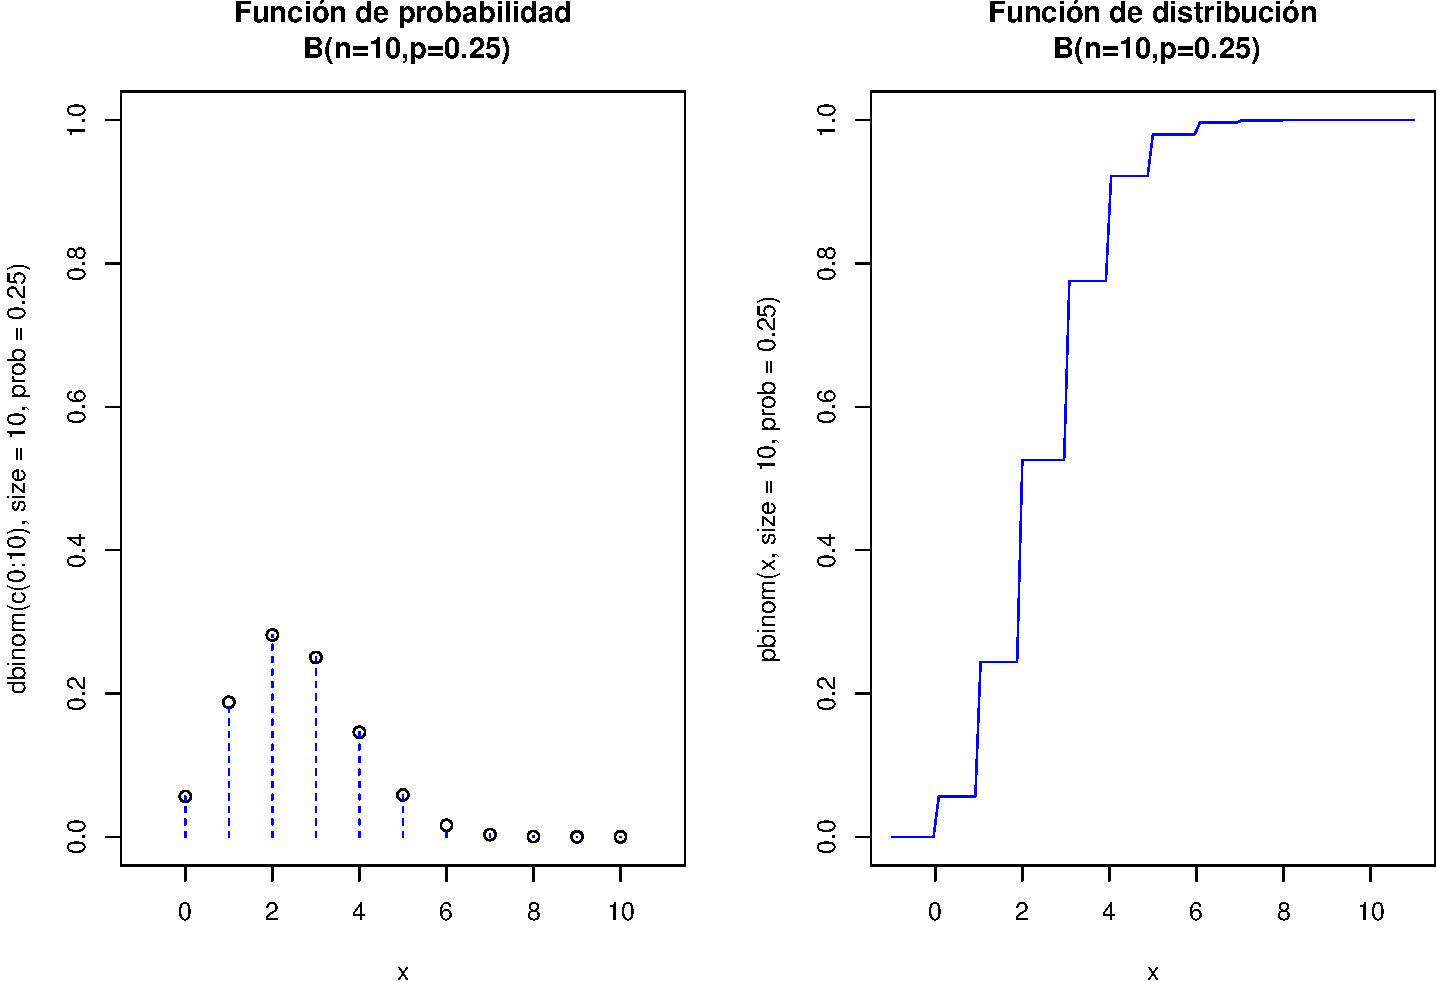
\includegraphics[width=0.7\linewidth]{Tema_4_Momentos_files/figure-beamer/unnamed-chunk-9-1}
\end{frame}

\begin{frame}{Método de rechazo}
\protect\hypertarget{muxe9todo-de-rechazo-2}{}
Para generar una \textbf{muestra aleatoria} de la variable \(X\),
hacemos lo siguiente:

\begin{enumerate}
[1)]
\item
  generamos un valor aleatorio \(x\) entre \(a\) y \(b\).
\item
  generamos un valor aleatorio \(y\) entre \(c\) y \(d\).
\item
  si \(y\leq f_X(x)\), aceptamos \(x\) como valor de la muestra. En caso
  contrario, volvemos a empezar en 1.
\end{enumerate}
\end{frame}

\begin{frame}{Ejemplo}
\protect\hypertarget{ejemplo-8}{}
\textbf{Ejemplo}

El gráfico de la figura anterior corresponde a la función de densidad
siguiente: \[
f_X(x)=\begin{cases}
x, & \mbox{ si }0\leq x\leq 1,\\
2-x, & \mbox{ si }1\leq x\leq 2,\\
0, & \mbox{en caso contrario.}
\end{cases}
\]
\end{frame}

\begin{frame}[fragile]{Ejemplo}
\protect\hypertarget{ejemplo-9}{}
Vamos a generar una muestra de \(25\) valores usando el \textbf{método
del rechazo}:

\begin{Shaded}
\begin{Highlighting}[]
\NormalTok{a}\OtherTok{=}\DecValTok{0}\NormalTok{; b}\OtherTok{=}\DecValTok{2}\NormalTok{; c}\OtherTok{=}\DecValTok{0}\NormalTok{; d}\OtherTok{=}\DecValTok{1}\NormalTok{; n}\OtherTok{=}\DecValTok{25}\NormalTok{; i}\OtherTok{=}\DecValTok{1}\NormalTok{;}
\NormalTok{f }\OtherTok{=} \ControlFlowTok{function}\NormalTok{(x)\{}\FunctionTok{ifelse}\NormalTok{(x}\SpecialCharTok{\textgreater{}=}\DecValTok{0} \SpecialCharTok{\&}\NormalTok{ x}\SpecialCharTok{\textless{}=}\DecValTok{1}\NormalTok{,x,}\FunctionTok{ifelse}\NormalTok{(x}\SpecialCharTok{\textgreater{}=}\DecValTok{1}\SpecialCharTok{\&}\NormalTok{x}\SpecialCharTok{\textless{}=}\DecValTok{2}\NormalTok{,}\DecValTok{2}\SpecialCharTok{{-}}\NormalTok{x,}\DecValTok{0}\NormalTok{))\}}
\NormalTok{muestra}\OtherTok{=}\FunctionTok{c}\NormalTok{()}
\ControlFlowTok{while}\NormalTok{(i }\SpecialCharTok{\textless{}=}\NormalTok{n)\{}
\NormalTok{  x}\OtherTok{=}\FunctionTok{runif}\NormalTok{(}\DecValTok{1}\NormalTok{,a,b)}
\NormalTok{  y}\OtherTok{=}\FunctionTok{runif}\NormalTok{(}\DecValTok{1}\NormalTok{,c,d)}
  \ControlFlowTok{if}\NormalTok{(y }\SpecialCharTok{\textless{}=} \FunctionTok{f}\NormalTok{(x))\{muestra}\OtherTok{=}\FunctionTok{c}\NormalTok{(muestra,x); i}\OtherTok{=}\NormalTok{i}\SpecialCharTok{+}\DecValTok{1}\NormalTok{\}}
\NormalTok{\}}
\NormalTok{muestra}
\end{Highlighting}
\end{Shaded}

\begin{verbatim}
 [1] 0.8934245 1.0241151 0.7485943 1.1318743 1.1174486 0.8956145 1.6270601
 [8] 0.6737312 0.9584882 0.5762514 0.7390811 0.4276671 1.5210227 0.8506008
[15] 0.4126257 0.9897587 1.2166050 1.6098125 0.8727734 0.8756381 1.4853939
[22] 1.1539542 1.2353779 0.5157756 1.2873756
\end{verbatim}
\end{frame}

\begin{frame}[fragile]{Ejemplo}
\protect\hypertarget{ejemplo-10}{}
Como hicimos con el ejemplo del \textbf{método de transformación}, vamos
a generar una muestra de 500 valores de la variable \(X\), vamos a
dibujar el \textbf{histograma de frecuencias relativas} junto con la
función de densidad para ver si ésta se aproxima a dicho histograma:

\begin{Shaded}
\begin{Highlighting}[]
\NormalTok{a}\OtherTok{=}\DecValTok{0}\NormalTok{; b}\OtherTok{=}\DecValTok{2}\NormalTok{; c}\OtherTok{=}\DecValTok{0}\NormalTok{; d}\OtherTok{=}\DecValTok{1}\NormalTok{; n}\OtherTok{=}\DecValTok{500}\NormalTok{; i}\OtherTok{=}\DecValTok{1}\NormalTok{;}
\NormalTok{f }\OtherTok{=} \ControlFlowTok{function}\NormalTok{(x)\{}\FunctionTok{ifelse}\NormalTok{(x}\SpecialCharTok{\textgreater{}=}\DecValTok{0} \SpecialCharTok{\&}\NormalTok{ x}\SpecialCharTok{\textless{}=}\DecValTok{1}\NormalTok{,x,}\FunctionTok{ifelse}\NormalTok{(x}\SpecialCharTok{\textgreater{}=}\DecValTok{1}\SpecialCharTok{\&}\NormalTok{x}\SpecialCharTok{\textless{}=}\DecValTok{2}\NormalTok{,}\DecValTok{2}\SpecialCharTok{{-}}\NormalTok{x,}\DecValTok{0}\NormalTok{))\}}
\NormalTok{muestra}\OtherTok{=}\FunctionTok{c}\NormalTok{()}
\ControlFlowTok{while}\NormalTok{(i }\SpecialCharTok{\textless{}=}\NormalTok{n)\{}
\NormalTok{  x}\OtherTok{=}\FunctionTok{runif}\NormalTok{(}\DecValTok{1}\NormalTok{,a,b)}
\NormalTok{  y}\OtherTok{=}\FunctionTok{runif}\NormalTok{(}\DecValTok{1}\NormalTok{,c,d)}
  \ControlFlowTok{if}\NormalTok{(y }\SpecialCharTok{\textless{}=} \FunctionTok{f}\NormalTok{(x))\{muestra}\OtherTok{=}\FunctionTok{c}\NormalTok{(muestra,x); i}\OtherTok{=}\NormalTok{i}\SpecialCharTok{+}\DecValTok{1}\NormalTok{\}}
\NormalTok{\}}
\FunctionTok{hist}\NormalTok{(muestra,}\AttributeTok{freq=}\ConstantTok{FALSE}\NormalTok{,}\AttributeTok{main=}\StringTok{"Histograma de la muestra"}\NormalTok{)}
\NormalTok{x2}\OtherTok{=}\FunctionTok{seq}\NormalTok{(}\AttributeTok{from=}\DecValTok{0}\NormalTok{,}\AttributeTok{to=}\DecValTok{2}\NormalTok{,}\AttributeTok{by=}\FloatTok{0.01}\NormalTok{)}
\FunctionTok{lines}\NormalTok{(x2,}\FunctionTok{f}\NormalTok{(x2),}\AttributeTok{col=}\StringTok{"red"}\NormalTok{)}
\end{Highlighting}
\end{Shaded}
\end{frame}

\begin{frame}{Ejemplo}
\protect\hypertarget{ejemplo-11}{}
\includegraphics[width=0.7\linewidth]{Tema_4_Momentos_files/figure-beamer/unnamed-chunk-12-1}
\end{frame}

\hypertarget{entropuxeda}{%
\section{Entropía}\label{entropuxeda}}

\begin{frame}{Introducción}
\protect\hypertarget{introducciuxf3n-3}{}
La \textbf{entropía} es una medida de la \textbf{incertidumbre} en un
experimento aleatorio.

Veremos cómo la \textbf{entropía} cuantifica la \textbf{incertidumbre}
por la cantidad de \textbf{información} requerida para especificar el
resultado de un experimento aleatorio.
\end{frame}

\begin{frame}{Entropía de una variable aleatoria}
\protect\hypertarget{entropuxeda-de-una-variable-aleatoria}{}
Supongamos que tenemos una variable aleatoria \(X\) discreta con valores
enteros: \(D_X=\{1,2,\ldots,N\}\).

Sea \(k\in D_X\) un valor de la variable. Estamos interesados en
cuantificar la \textbf{incertidumbre} del suceso \(A_k =\{X=k\}\).

O sea, cuánta \textbf{menos incertidumbre} tenga \(A_k\), más
\textbf{alta será su probabilidad}, y cuánta \textbf{más incertidumbre},
\textbf{menos probabilidad} de aparecer \(A_k\).
\end{frame}

\begin{frame}{Entropía de una variable aleatoria}
\protect\hypertarget{entropuxeda-de-una-variable-aleatoria-1}{}
Una medida que cumple las condiciones anteriores es la siguiente:
\(I(A_k)=I(\{X=k\})=\ln\left(\frac{1}{P(X=k)}\right)=-\ln\left(P(X=k)\right).\)

Por ejemplo, si \(P(A_k)=1\), o sea, \(A_k\) aparece
``\textbf{seguro}'', entonces tiene incertidumbre \textbf{nula},
\(I(A_k)=0\), y si \(P(A_k)=0\), o sea, \(A_k\) no aparece
``\textbf{nunca}'', tiene incertidumbre \textbf{máxima},
\(I(A_k)=\infty\).
\end{frame}

\begin{frame}{Entropía de una variable aleatoria}
\protect\hypertarget{entropuxeda-de-una-variable-aleatoria-2}{}
La motivación anterior hace que definamos la \textbf{entropía} de una
variable aleatoria de la forma siguiente:

Definición: Sea \(X\) una variable aleatoria con función de densidad
\(f_X(x)\) en el caso continuo o función de probabilidad \(P_X(x)\) en
el caso discreto. Definimos \textbf{entropía de X} como:
\(H_X = E\left(-\ln(f_X)\right)=\int_{-\infty}^\infty -\ln(f_X(x)) f_X(x)\, dx,\)
en el caso continuo y,
\(H_X = E\left(-\ln(P_X)\right)=\sum_{x_k\in D_X} -\ln(P_X(x_k)) P_X(x_k),\)
en el caso discreto.
\end{frame}

\begin{frame}{Ejemplo}
\protect\hypertarget{ejemplo-12}{}
\textbf{Ejemplo: entropía de una variable de Bernoulli de parámetro
\(p\)}

Sea \(X\) una variable de Bernoulli de parámetro \(p\).

Recordemos que su función de probabilidad \(P_X\) es: \(P_X(0)=1-p=q,\)
\(P_X(1)=p\).

La entropía de \(X\) será: \[
H_X = E\left(-\ln(P_X)\right) = -(1-p)\cdot \ln(1-p)-p\cdot \ln p.
\] El gráfico de la entropía se puede observar en el gráfico siguiente
donde \(X\) tiene entropía máxima cuando \(p=\frac{1}{2}\) que sería
cuando \(X\) tiene incertidumbre máxima al tratar de adivinar el
resultado de \(X\) y \(X\) tiene entropía mínima cuando \(p=0\) o
\(p=1\) ya que en estos casos el resultado de \(X\) sería siempre \(0\)
o \(1\), respectivamente.
\end{frame}

\begin{frame}{Ejemplo}
\protect\hypertarget{ejemplo-13}{}
\textbf{Ejemplo: entropía de una variable de Bernoulli de parámetro
\(p\)}

\includegraphics[width=0.7\linewidth]{Tema_4_Momentos_files/figure-beamer/unnamed-chunk-13-1}
\end{frame}

\begin{frame}{Ejemplo}
\protect\hypertarget{ejemplo-14}{}
\textbf{Entropía de una variable aleatoria exponencial de parámetro
\(\lambda\)}

Sea \(X\) una variable aleatoria exponencial de parámetro \(\lambda\).

Recordemos que su función de densidad es:
\(f_X(x)=\lambda \mathrm{e}^{-\lambda x}\), si \(x\geq 0\) y
\(f_X(x)=0\), en caso contrario.

Su entropía será: \[
\begin{array}{rl}
H_X & = E\left(-\ln(f_X)\right)=-\int_0^\infty \ln\left(\lambda\mathrm{e}^{-\lambda x}\right)\lambda\mathrm{e}^{-\lambda x}\, dx = -\lambda \int_0^\infty (\ln(\lambda) -\lambda x)\mathrm{e}^{-\lambda x}\, dx \\ & = -\ln (\lambda)\int_0^\infty \lambda\mathrm{e}^{-\lambda x}\, dx+\lambda \int_0^\infty \lambda x \mathrm{e}^{-\lambda x}\, dx =-\ln(\lambda)\int_0^\infty f_X(x)\, dx +\lambda E(X)\\ & =-\ln(\lambda)+\lambda \frac{1}{\lambda} =1-\ln(\lambda).
\end{array}
\] El gráfico de la entropía se puede observar en el gráfico siguiente
donde \(X\) tiene entropía máxima cuando \(\lambda=0\) que sería cuando
\(X\) tiene incertidumbre máxima al tratar de adivinar el resultado de
\(X\) al tener media \(E(X)=\frac{1}{\lambda}=\infty\) y \(X\) tiene
entropía mínima cuando \(\lambda\) tiende a \(\infty\) ya que su media
\(E(X)=\frac{1}{\lambda}\) tendería a 0.
\end{frame}

\begin{frame}{Ejemplo}
\protect\hypertarget{ejemplo-15}{}
\textbf{Ejemplo: entropía de una variable exponencial de parámetro
\(\lambda\)}

\includegraphics[width=0.7\linewidth]{Tema_4_Momentos_files/figure-beamer/unnamed-chunk-14-1}
\end{frame}

\end{document}
